\documentclass{CUP-JNL-DTM}
\DeclareUnicodeCharacter{274C}{\texttimes}
%%%% Packages
\usepackage{graphicx}
\usepackage{multicol,multirow}
\usepackage{amsmath,amssymb,amsfonts}
\usepackage{mathrsfs}
\usepackage{amsthm}
\usepackage{rotating}
\usepackage{appendix}
% For JDM please remove the natbib package:
\usepackage[numbers]{natbib}
% And use biblatex-apa with a .bib file to format your references according to the APA7 style.
% \usepackage[natbib,style=apa]{biblatex}
% \addbibresource{your-refs.bib}
\usepackage{ifpdf}
\usepackage[T1]{fontenc}
\usepackage{newtxtext}
\usepackage{newtxmath}
\usepackage{textcomp}
\usepackage{xcolor}
\usepackage{lipsum}
\usepackage{listings}
\usepackage[colorlinks,allcolors=blue]{hyperref}
\newtheorem{theorem}{Theorem}[section]
\newtheorem{lemma}[theorem]{Lemma}
\theoremstyle{definition}
\newtheorem{remark}[theorem]{Remark}
\newtheorem{example}[theorem]{Example}
\numberwithin{equation}{section}
\usepackage{longtable} % For tables that span multiple pages
\usepackage{array}     % To create more flexible tables

\artid{01}
\jname{}
\jvol{00}
\jissue{00}
\jyear{{2025}}
\jmonth{03}
%\artid{20}
%\jvol{4}
%\jissue{1}
%\raggedbottom


\begin{document}

\begin{Frontmatter}

\title[Article Title]{Learning to See Similarity: Deep Metric Embeddings for Pet Breed Recognition
}

% There is no need to include ORCID IDs in your .pdf; this information is captured by the submission portal when a manuscript is submitted. 
\author[1]{Paulo Henrique da Silva Mota}

\address[1]{\orgdiv{Division}, \orgname{OPIT - Open Institute of Technology}, \orgaddress{\city{St. Julian’s},  \country{Malta}}. \email{paulo.d@students.opit.com}}


\end{Frontmatter}

\section{Introduction}
\paragraph{}This report details the development of a deep learning model for understanding the visual relationships between different pet breeds. Instead of just classifying each image with a single breed label, we focus on learning an embedding space. In this space, images of pets that look alike will be located close to each other, while images of different-looking pets will be further apart. This approach is useful in applications like finding similar images and identifying breeds with limited examples.

We will train a convolutional neural network (CNN) to create these embeddings using images from the Oxford-IIIT Pet Dataset, which contains pictures of 37 breeds of cats and dogs. To evaluate how well the model learns, we will perform several tasks: checking if two images show the same breed, retrieving the most similar images to a given one, and classifying breeds when only a few examples are available. Finally, we will visualize the learned embedding space to see how the different breeds are organized based on their visual similarities.

\section{Metric Learning Pipeline}

\paragraph{}We defined a model training pipeline for learning embeddings using a CNN backbone (defaulting to ResNet18) followed by a projection head. It employs the TripletMarginLoss along with TripletMarginMiner to train the network to produce embeddings where similar samples are close and dissimilar ones are far apart, optimized using the Adam algorithm. The training loop iterates through epochs, calculating the loss on hard triplets and updating the model's weights, then visualizing the training loss over time.

\begin{figure}[ht]
    \centering
    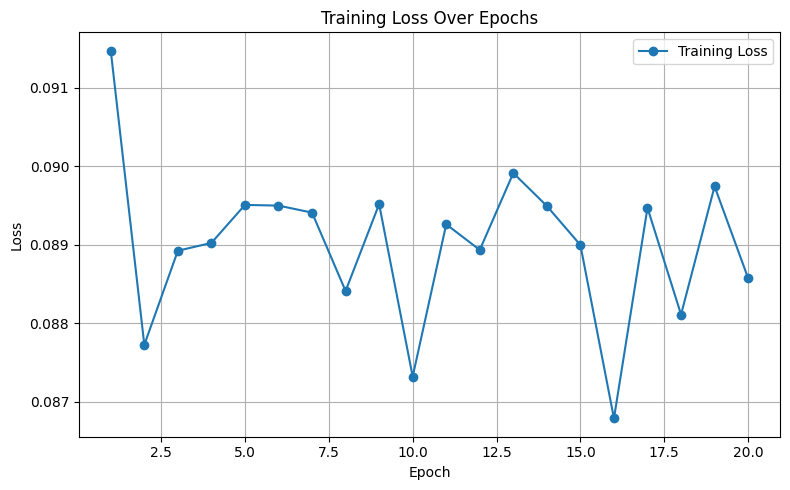
\includegraphics[width=0.5\linewidth]{loss.png}
    \caption{Model training Loss over epochs}
    \label{fig:enter-label}
\end{figure}


\newpage

\section{Verification Task}

\paragraph{}The embedding system's verification performance was evaluated by creating numerous pairs of embeddings, some from the same identity and others from different identities. The function then calculated the distances between the embeddings in each pair, operating on the principle that embeddings of the same identity should be closer than those of different identities. By comparing these distances to the known identities, the system's ability to correctly classify pairs as belonging to the same or different identities was assessed, leading to the calculation of key performance metrics.

\paragraph{}The results of this evaluation are highly positive. The ROC-AUC of 0.9759 signifies excellent overall discriminative power, indicating that the embeddings effectively separate instances of the same identity from different ones across various decision thresholds. Furthermore, the low Equal Error Rate (EER) of 0.0711 suggests a good balance between false acceptances and false rejections at a practical operating point. These metrics collectively demonstrate that the embedding system performs very well in verifying identities, accurately capturing the distinguishing characteristics of the data.


\begin{figure}[ht]
    \centering
    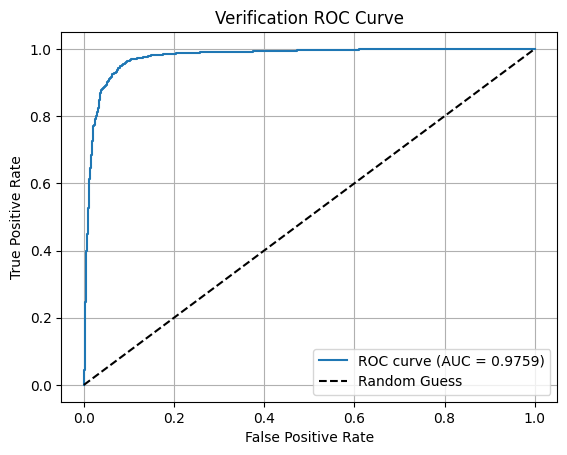
\includegraphics[width=0.6\linewidth]{roccurve.png}
    \caption{Verification ROC Curve}
    \label{fig:enter-label}
\end{figure}

\section{Retrieval Task}

\paragraph{}We assesses the performance of a retrieval system using embeddings. Taking query embeddings and their corresponding labels, along with a larger set of all embeddings and their labels. Our function employs a k-Nearest Neighbors (KNN) algorithm to find the \verb|k| most similar embeddings in the entire dataset for each query embedding based on their Euclidean distance.

\paragraph{}For each specified value of \verb|k| (e.g., 1 and 5), the function calculates the retrieval accuracy. It determines how many of the \verb|k| nearest neighbors retrieved for each query embedding share the same label as the query. From this, it computes two key metrics: Recall@k, which measures the proportion of relevant items (same label) retrieved within the top \verb|k| results, and Precision@k, which measures the proportion of retrieved items within the top \verb|k| that are relevant.

\paragraph{}The evaluation yielded the following results:

\begin{itemize}
    \item \textbf{Recall@1: 0.7912} and \textbf{Precision@1: 0.7912}: When considering only the single nearest neighbor (k=1), the system retrieved a relevant item (an embedding with the same label as the query) 79.12\% of the time. Since only one item is retrieved, precision and recall are the same in this case.
    \item \textbf{Recall@5: 3.8885} and \textbf{Precision@5: 0.7777}: When considering the top 5 nearest neighbors (k=5), on average, 3.8885 relevant items were found within these top 5 for each query. The precision at 5 indicates that out of all the retrieved items in the top 5 across all queries, 77.77\% of them had the correct label.
\end{itemize}
\paragraph{}These metrics indicate a strong retrieval performance. At k=1, there's a high chance of retrieving the correct match as the nearest neighbor. While Recall@5 increases (as expected, since more items are considered), Precision@5 remains high, suggesting that a large proportion of the top 5 retrieved items are relevant to the query. The function further visualizes the precision and recall at different \verb|k| values using a bar chart.

\begin{figure}[ht]
    \centering
    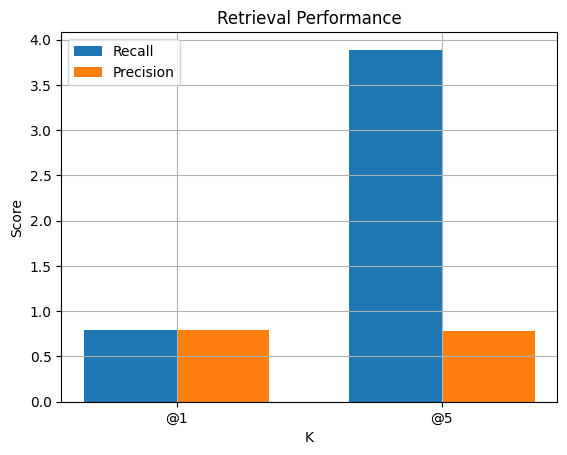
\includegraphics[width=0.6\linewidth]{retrivals.png}
    \caption{Retrieval Performance}
    \label{fig:enter-label}
\end{figure}

\section{Few-shot Classification}

 \paragraph{}The few-shot evaluation involves creating numerous distinct learning tasks. In each task, the system is presented with a small number of labeled support examples from novel classes and is then challenged to correctly classify a set of unseen query examples from the same classes. For each task, a subset of classes is randomly chosen, and a support set (containing a few labeled instances per class) and a query set (containing new, unlabeled instances from those same classes) are constructed. A Nearest Neighbor classifier is trained on the support set to predict the labels of the query set, and the accuracy of these predictions is recorded.

The evaluation of this few-shot classification approach yielded a high mean accuracy of 0.9575 with a low standard deviation of 0.0439 across the simulated tasks. This indicates that, on average, the system correctly classified approximately 95.75\% of the unseen query examples in each few-shot scenario. The small standard deviation suggests that the system's performance is remarkably consistent across different sets of novel classes and their limited support examples. These results demonstrate a very strong capability for few-shot learning, highlighting the effectiveness of the underlying data embeddings in enabling rapid generalization to new, unseen categories from only a few labeled instances.


\begin{figure}[ht]
    \centering
    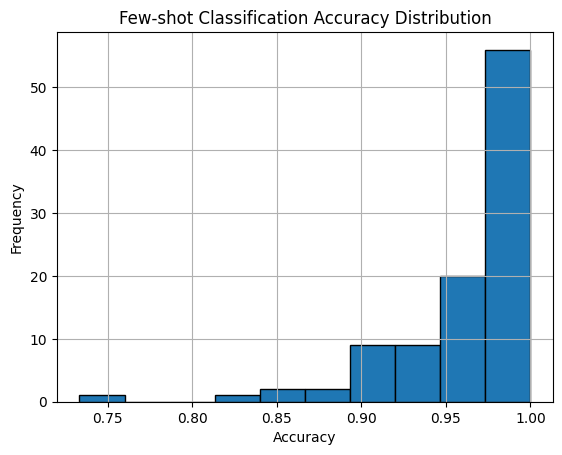
\includegraphics[width=0.75\linewidth]{rttttttttttt.png}
    \caption{Accuracy distribution for few-shot classification}
    \label{fig:enter-label}
\end{figure}

\section{Embedding Space Visualization}

\paragraph{}Providing a visual representation of high-dimensional embeddings in a lower-dimensional space, specifically focusing on a user-selected subset of classes. It begins by identifying the indices corresponding to the chosen class names within the provided list of all class names. Then, it filters the input embeddings and their labels to include only the data points belonging to these selected classes.

If there are enough data points for the selected classes (more than the desired number of reduced dimensions), the function applies the t-distributed Stochastic Neighbor Embedding (t-SNE) algorithm. t-SNE is a dimensionality reduction technique particularly well-suited for visualizing high-dimensional datasets in two or three dimensions while preserving the local structure of the data. The reduced embeddings are then plotted on a scatter plot, with each point colored and labeled according to its original class. This visualization allows for an inspection of how well the embeddings cluster based on their class membership, providing insights into the separability of the chosen classes in the embedding space. If there are insufficient samples for the selected classes, a message is printed indicating this limitation.

\begin{figure}[ht]
    \centering
    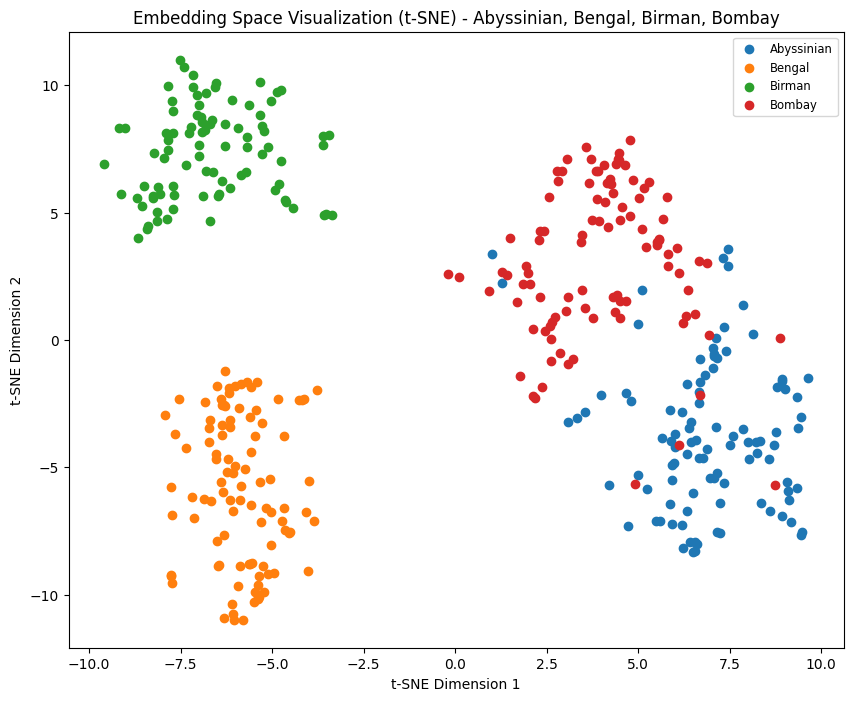
\includegraphics[width=0.75\linewidth]{scatter22.png}
    \caption{Embedding Space Visualization (t-SNE)}
    \label{fig:enter-label}
\end{figure}

\nocite{*} % This forces all references to be shown, even if not cited

\newpage

\section{References} 
\renewcommand{\refname}{} % Remove References 
\begin{thebibliography}{99}

\bibitem{MusgravePytorchMetricLearning}
Kevin Musgrave, Serge Belongie, and Vittorio Ferrari,
\emph{PyTorch Metric Learning},
\url{https://kevinmusgrave.github.io/pytorch-metric-learning/} (accessed: 2025-04-26)

\bibitem{noauthor_oxfordiiitpet_nodate} 
OxfordIIITPet — Torchvision main documentation, \url{https://pytorch.org/vision/main/generated/torchvision.datasets.OxfordIIITPet.html} (accessed: 2025-03-02).

\bibitem{noauthor_how_2020} 
How ReLU and Dropout Layers Work in CNNs | Baeldung on Computer Science, \url{https://www.baeldung.com/cs/ml-relu-dropout-layers}, 2020-05-30 (accessed: 2025-03-02).

\bibitem{noauthor_nvidia_nodate} 
NVIDIA A100 GPUs Power the Modern Data Center, \url{https://www.nvidia.com/en-us/data-center/a100/} (accessed: 2025-03-02).

\bibitem{noauthor_google_nodate} 
Google Colab, \url{https://research.google.com/colaboratory/faq.html} (accessed: 2025-03-02).




\end{thebibliography}


\end{document}
